\chapter{Теоретическая часть}
\section{Полупроводник}
Рассматривая полупродники, мы будем говорить о кристалических телах. Для анализа таких тел необходимо решить уравнение Шредингера для нахождения, к примеру, энергитеских уровней. В целях упрощения задачи и сохранения наиболее характерных черт системы в Зонной теории вводится ряд допущений \cite{Kalashnikov}: 
\begin{enumerate}
	\item Атомные ядра являются неподвижными источниками поля, действующего на электроны;
	\item Расположения атомных ядер в пространстве является строго переодичным: они распологаются в узлах идеальной кристалической решетки;
	\item Взаимодейсвие электронов друг с другом заменяется некоторым внешним полем.
\end{enumerate}

\subsection{Зонная структура}
В следствии симметрии и переодичности идеального кристалла по разлиным направлениям и теории Блоха, для описания дисперсии электронов используют зоны Бриллюэна. Так как закон дисперсии переодичен на всем кристалле, для его описания можно использовать только первую зону Бриллюэна. 
\begin{figure}[h]
	\centering
    \begin{minipage}[b]{0.5\textwidth}
	    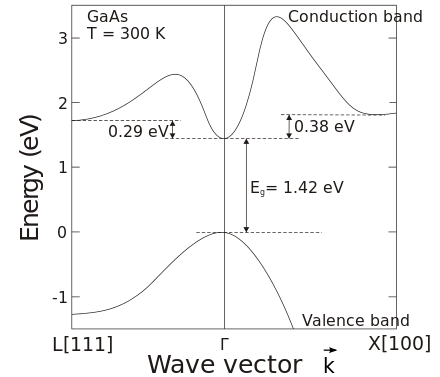
\includegraphics[width=0.9\textwidth]{assets/GaAs_E}
	    \caption{Зонная структура $GaAs$}
	\end{minipage}
	\hfill
	\begin{minipage}[b]{0.45\textwidth}
		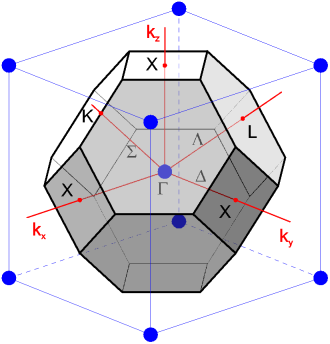
\includegraphics[width=0.8\textwidth]{assets/ZnLaer}
	    \caption{Элементарная ячейка типа Цинковой обманки}
	\end{minipage}
\end{figure}

\subsection{Зонная диаграмма}
Для наглядного представления и сравнения полупроводников и других материалов удобно использовать зонную диаграмму (рис.~\ref{img:Zone}).
\begin{figure}
	\centering
	\includegraphics[width=\textwidth]{assets/Zone}
    \caption{Характерный вид зонной диаграммы для различных материалов}
    \label{img:Zone}
\end{figure}\\
\begin{conditions}
	$E_{c}$ & дно зоны проводимости (ЗП);\\
	$E_{v}$ & потолок валентной зоны (ВЗ);\\
	$E_{F}$ & уровень (квазиуровень) Ферми;\\
	$E_{g}$ & запрещенная зона (ЗЗ);\\
	$\chi$ & электронное сродство;\\
	$\varphi$ & работа выхода.
\end{conditions}
\begin{center}
  \begin{longtable}{|c|c|}
    \caption{Основные параметры $Al_{x}Ga_{1−x}As$}
    \label{tab:2.0.0}
    \\ \hline
    Параметр & $Al_{x}Ga_{1−x}As$ \\
    \hline \endfirsthead
    \subcaption{Продолжение таблицы~\ref{tab:2.0.0}}
    \\ \hline \endhead
    \hline \subcaption{Продолжение на след. стр.}
    \endfoot
    \hline \endlastfoot
	Кристаллическая структура& Типа цинковой обманки \\ \hline
	Постоянная решетки $a[nm]$  & $0.56533+0.00078x$ \\ \hline
	$E_{g}^{\Gamma}[eV],\, x < 0.45$    & $1.424+1.247x$ \\ \hline
	$E_{g}^{\Gamma}[eV],\, x > 0.45$    & $1.656+0.215x+0.143x^{2}$ \\ \hline
	% $\Delta E_{c}^{\Gamma}[eV],\, x < 0.45$    & $0.773x$ \\ \hline
	% $\Delta E_{c}^{\Gamma}[eV],\, x > 0.45$    & $0.232-0.259x+1.147x^{2}$ \\ \hline
	$m_{e}^{\Gamma}$    & $0.067+0.083x$ \\ \hline
	$m_{lh}$    & $0.082+0.071x$ \\ \hline
	$N_{atoms}[1/sm^{-3}]$    & $(4.42-0.17x)10^{22}$
  \end{longtable}
\end{center}

\subsection{Плотсноть состояний}

\subsection{Концентрация носителей заряда}

\subsubsection{Собственный полупроводник}

\subsubsection{Легированный полупроводник}
